%Chapter 3

\renewcommand{\thechapter}{3}
\newcommand{\KrCal}{$\rm^{83m}Kr \: $}


\chapter{XYZ Correction}
\label{Ch:3}

\section{$\rm^{83m}Kr$ Calibration}

Throughout the science run periodic $\rm^{83m}Kr$ injections were performed and used to calculate position dependent corrections. $\rm ^{83m}Kr$ is produced from the decay $\rm^{83}Rb$ with a half life of 86.2 days, the $\rm^{83}Rb$ source we use is housed in charcoal and plumed into the LUX circulation system. The daughter \KrCal is continually produced in the charcoal housing, having a half-life 1.8 hours. $\rm^{83m}Kr$ decays via an electron capture first emitting a 32.1 [keV] gamma followed by a 9.4 [keV] with a half life of 154 [ns] between the two (refs). The combined S1 pulse corresponding to (41.55 [keV]) is observed in LUX the for the majority of the decays since the minimum S1 pulse separation is set to 1000 [ns]. The \KrCal source is introduced when needed into the LUX detector by flushing the charcoal housing with xenon and diverting the flow inline with the main circulation path. The \KrCal source and delivery into the xenon detector is described in more detail in ref[Kastins]. The relatively short half-life of 1.8 hours allows for several injections per week without interrupting WIMP search data taking. Once injected the source is uniformly mixed into the liquid xenon within a matter of minutes and can be used to calculate corrections for the XYZ the response of the detector. The combined gammas from the decays are observed as a single pulse providing a powerful tool for tracking the detector response in x,y,z over the course of the science run. Figure \ref{fig:Kr_Dist} shows the uniform distribution of \KrCal events in the LUX detector thirty minutes after the injection. The better we can correct for position dependance of the S1 and S2 signals the smaller the observed fluctuations will be, leading to better ER, NR discrimination and ultimately better signal to background for the WIMP search.


\begin{figure}[h!]\centering
\includegraphics[width=72mm]{Chapter_XYZ_Corr/Thesis_Corr_Plots/Kr_XY_density.png}
\includegraphics[width=72mm]{Chapter_XYZ_Corr/Thesis_Corr_Plots/Kr_RZ_density.png}
\caption{Distribution of \KrCal events 10 minutes after the injection. The source readily mixed uniformly throughout the liquid xenon illuminating all regions of the active volume. The solid black lines represent the fiducial volume used for the WIMP search. }
\label{fig:Kr_Dist}
\end{figure}



%uniform illumination.... show decay constant.

\section{S2 Electron Lifetime and x,y Correction}


The S1 and S2 signals collected on the top and bottom PMT arrays have accosted x,y,z positions computed from the S2 hit pattern (x,y) and the signal separation in time (z). Knowing the x,y,z position provides a powerful tool for reducing fluctuations in the signals due to detector geometry. The dominant effect to correct the data for is the free electron lifetime, as charge is drifted from the event site to the extraction region (0-47 cm) electronegative impurities in the liquid latch onto them. These impurities include residual $\rm O_2$, $\rm H_2O$, $\rm N_2$ in the xenon (1 ppb $\rm O_2$ corresponds to a 100 $\rm \mu s$ lifetime [ref]). Through the science run the electron lifetime was measured between 500 to 1000 $\rm \mu s$ (75 to 150 cm drift length), corresponding to between 70\% and 50\% reduction in S2 signal from the bottom of the detector. 
The electron lifetime is calculated by binning the detector in drift time into 60 z slices, in each bin a Gaussian is fit to extract the mean. We then fit an exponential to the mean S2 response vs. z to extract characteristic drift time $\lambda$ [$\rm \mu s$], shown in figure \ref{fig:S2_EL}. The electron lifetime extraction from a $\rm^{83}Kr$ data set is shown in figure 4.  For this analysis we use the S2 response on he bottom PMT array, defined as $\rm S2_b$, this convention is chosen since the light in the bottom PMT array is more uniformly distributed than on the top PMTs. Also, two PMTs are not bias on the top PMT arrays which could lead to a significant loss in S2 signal for a potential WIMP events extracted at the location of the unbiassed PMT.


\begin{figure}[h!]\centering
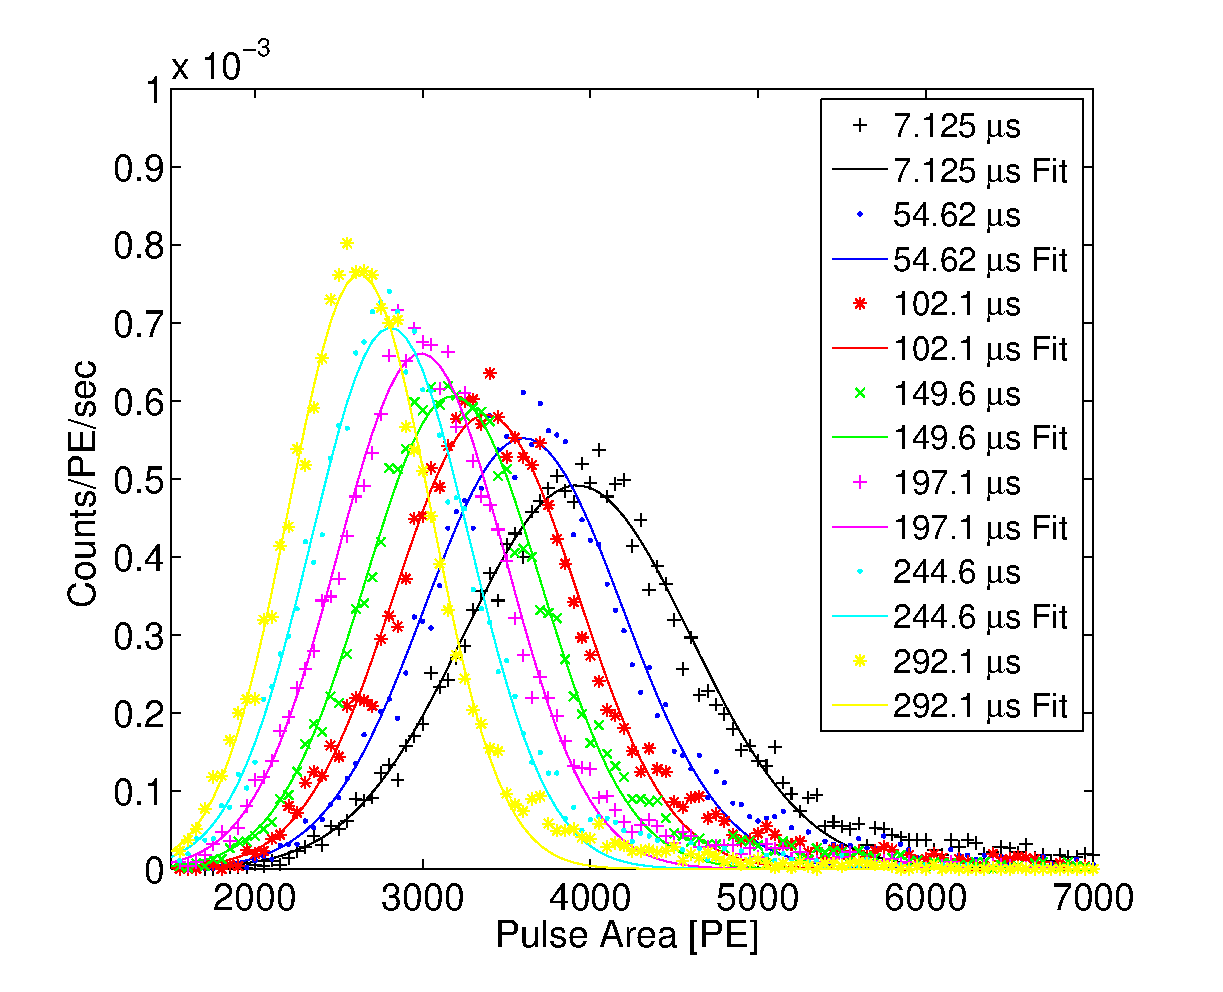
\includegraphics[width=75mm]{Chapter_XYZ_Corr/Thesis_Corr_Plots/S2_bottom_hist_EL.eps}
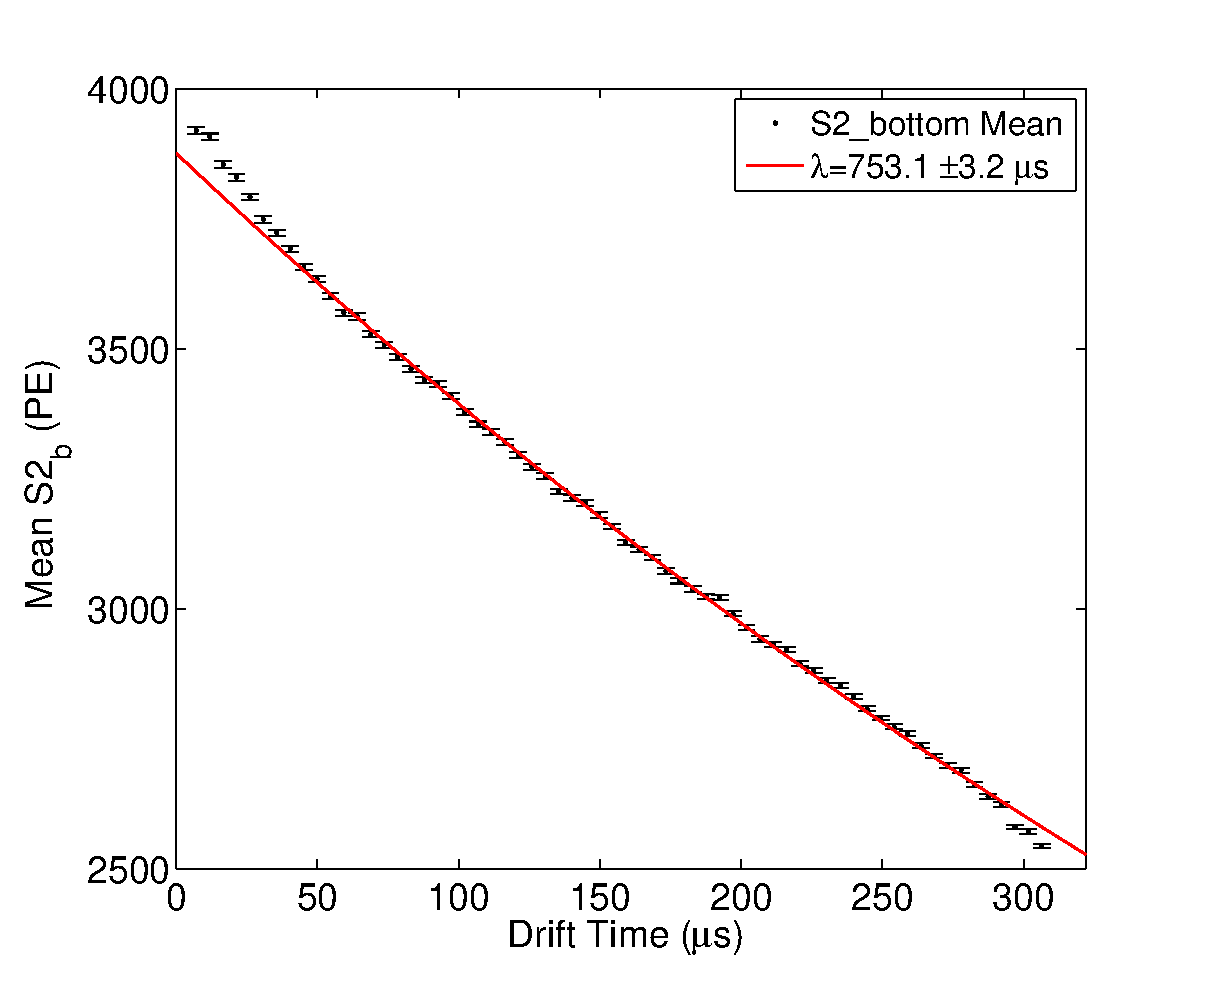
\includegraphics[width=73mm]{Chapter_XYZ_Corr/Thesis_Corr_Plots/S2_bottom_lifetime.eps}
\caption{Left: Fits to the mean of $\rm S2_b$ in several z slices. Right, the exponential fit to the means of $\rm S2_b$ vs. drift time used to extract electron lifetime $\rm \lambda$. }
\label{fig:S2_EL}
\end{figure}

The z corrected $\rm S2_b$ is calculated as follows:
\begin{equation}
\rm S2_{\operatorname{b-z}}=S2_b\cdot exp\left(\frac{drift\,time[\mu s]}{\lambda[\mu s]}\right)
\label{eq:S2_Z}
\end{equation}

Where $\rm S2_{\operatorname{b-z}}$ is the z corrected $\rm S2_b$ signal and $\rm \lambda$ is the free electron lifetime.

After correcting the dominant z dependent electron attenuation, corrected to 0 drift time, we calculate the normalization factor ($\mathcal{NF}$) that will be used to flat field the x,y dependance of the S2 signal. The S2 light is emitted when the charge is extracted from the liquid above the gate and is accelerated by a 6 kV potential to the anode, traversing 5mm. Fluctuations in x,y response to a given number of electrons are caused by non uniformities in the extraction field, tilt in the liquid level, and non uniformities in the anode-gate separation (potentially wire sagging). All these variations lead to additional fluctuations in the S2 signal, by using a the $\rm^{83m}Kr$ the response can be corrected as a function of  x,y position. The normalization is calculated by creating a 25x25 grid on the x,y plane, corresponding to 2[cm] x 2[cm] x,y bins, for each bin center the average light response is determined by fitting a Gaussian. Figure \ref{fig:S2_XY_norm_center} on the left, shows the measured $\rm S2_b$ response to 1 million $\rm^{83m}Kr$ decays normalized to the response at the center, x=y=0, this map represents the inverse of the normalization factor that we call $\rm\mathcal{NF}(x,y)$. $\mathcal{NF}$ is then applied to the $\rm S2_b$ data by using a spline interpolation of the x,y coordinate of each event relative to the bin centers $\rm\mathcal{NF}(x,y)$. Figure \ref{fig:S2_XY_norm_center} on the right, shows the $\rm S2_b$ response after flat fielding the data relative to the center x=y=0 using $\rm\mathcal{NF}(x,y)$. After applying the x,y correction the fluctuation decrease from 10\% to 1\% in the inner 18 cm of the detector (the fiducial volume).

%talk about the bins. 25x25 grid, or 50x 50 grid. (with at least 100 events each to define the mean with a Gaussian)

\begin{figure}[h!]\centering
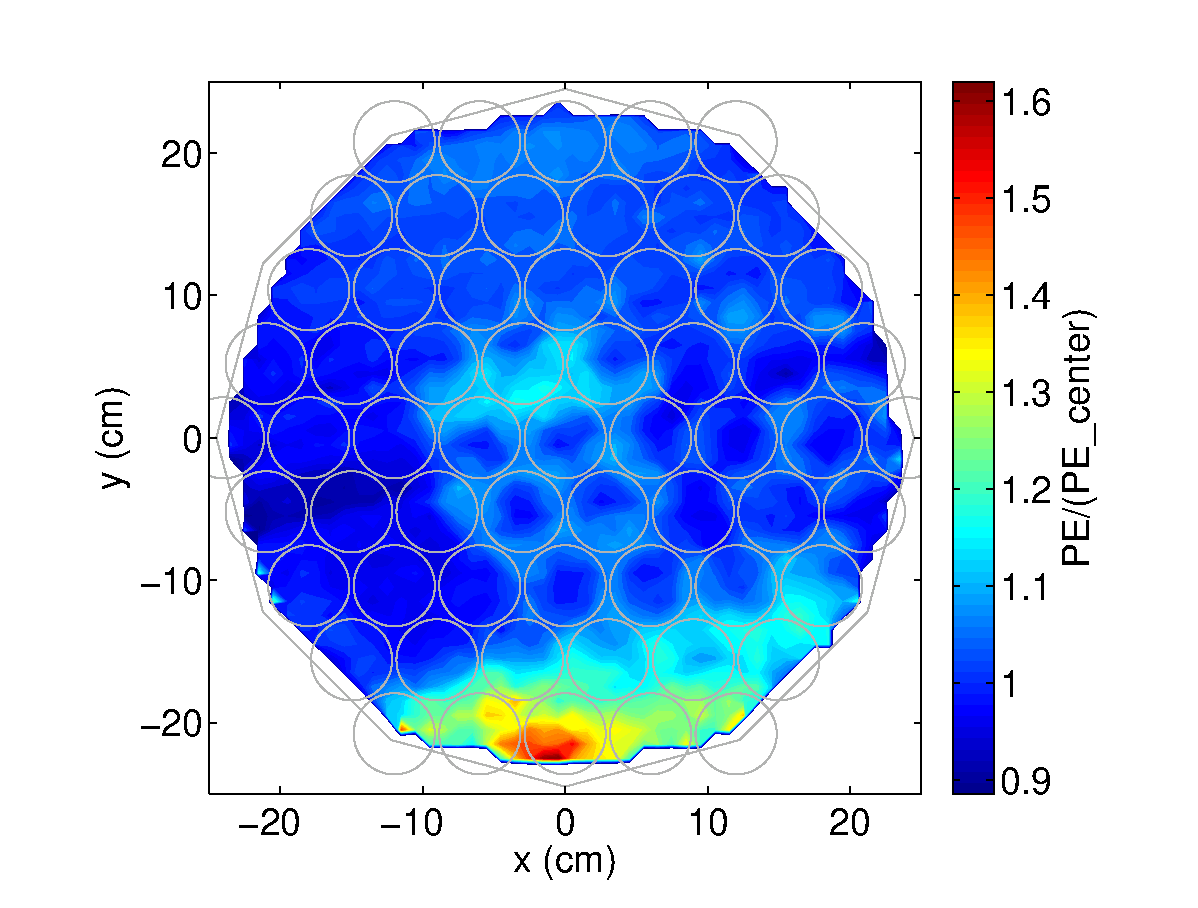
\includegraphics[width=74mm]{Chapter_XYZ_Corr/Thesis_Corr_Plots/S2_b_1cm_1cm/S2_b_XY_1cm_norm.eps}
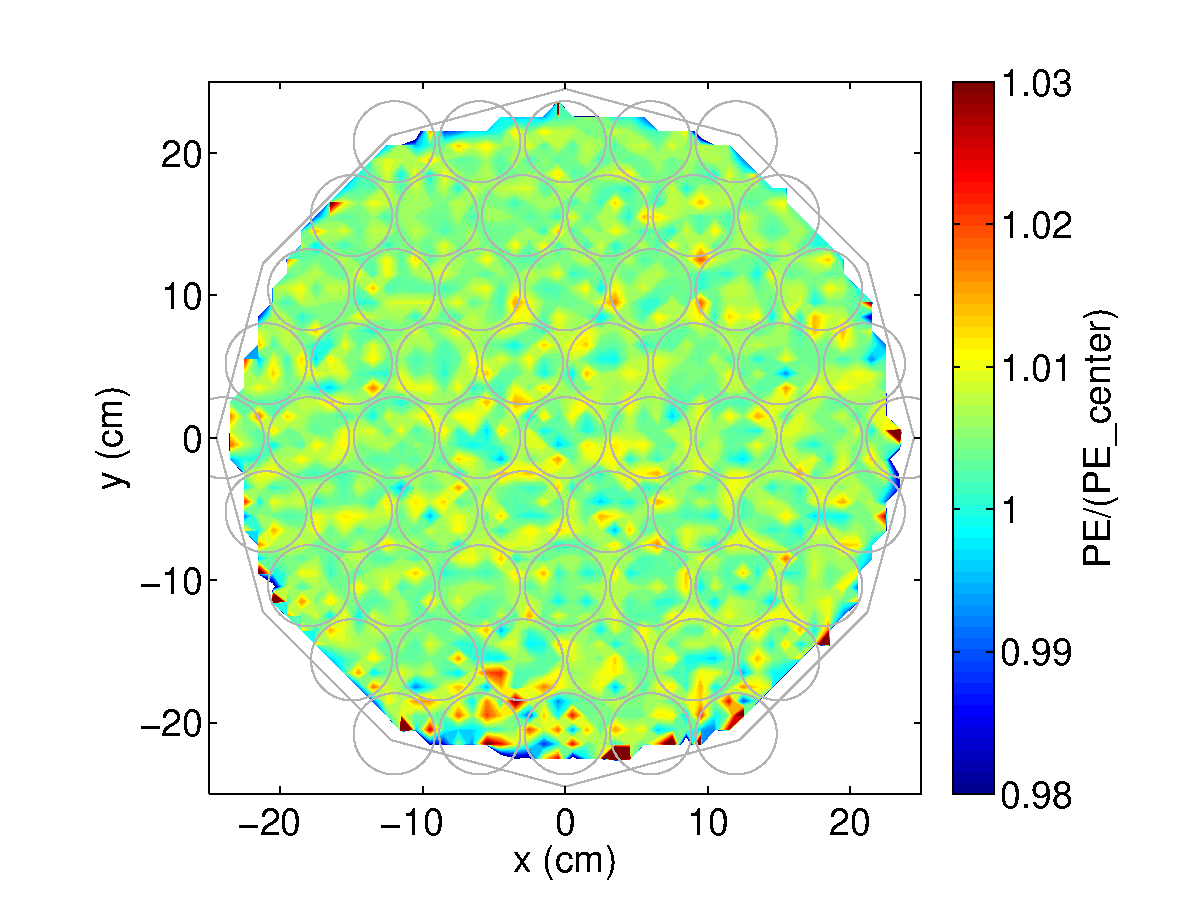
\includegraphics[width=74mm]{Chapter_XYZ_Corr/Thesis_Corr_Plots/S2_b_1cm_1cm/S2_b_XY_1cm_norm_FlatField.eps}
\caption{Left: Response of $\rm S2_b$ vs. x,y normalized to the response at the center (x=y=0). Right: Response of $\rm S2_b$ vs. x,y after flat fielding the data using $\rm\mathcal{NF}_{S2_b}$. }
\label{fig:S2_XY_norm_center}
\end{figure}


After correcting for z and x,y we can define the position dependent  (x,y,z) corrected $\rm S2_b$ signal, which we will call $\rm S2{_b}_c$ calculated as follows:
\begin{equation}
\rm S2_{\operatorname{b-c}}= S2_{\operatorname{b-(x,z,y)}}=S2_{\operatorname{b-z}} \cdot \mathcal{NF}_{S2_b}(x,y)
\label{eq:S2_XYZ}
\end{equation}

Where $\rm S2_{\operatorname{b-c}}$ is the x,y,z corrected $\rm S2_b$ signal and $\rm \mathcal{NF}_{S2_b}(x,y)$ is the Normalization Factor'of the bottom PMT array for S2s and is a function of x,y. The interpolation of the inverse of $\rm \mathcal{NF}_{S2_b}(x,y)$ along the x,y grid is plotted in figure \ref{fig:S2_XY_norm_center}.


After applying the z correction to $\rm S2_b$ there is an improvement in resolution of 18\%, for the case of an 750 $\rm \mu s$ electron lifetime. The flat fielding in the x,y plane provides an additional 4.9\% improvement in resolution to the $\rm S2_b$ signal. Figure \ref{fig:S2_res} shows the improvement in the $\rm S2_b$ signal after applying the z and x,y correction.

\begin{figure}[h!]\centering
\includegraphics[width=80mm]{Chapter_XYZ_Corr/Thesis_Corr_Plots/S2_corr_res.eps}
\caption{Improvement of resolution in $\rm S2_b$ after applying the z and x,y,z correction. }
\label{fig:S2_res}
\end{figure}



\section{S1 x,y,z Correction}

The S1 light propagates from the interaction sight, unlike the S2, and has about a 30\% variation in light collection efficiency between events near the top and bottom of the detector. About 2/3 of the S1 light is collected on the bottom PMT arrays due to total internal reflection at the liquid gas interface, and as events move closer to the bottom PMTs the probability of a photon stricking a PMT and producing a photo electron (PE) increases. Other position dependent effects include the photon absorption length which is negligible at the purities achieved in LUX and teflon reflectivity, about 95\%. Any quantum efficiency (QE) variations between the 122 PMTs that are properly normalized by the individual gain corrections are also folded into the S1 position dependent correction, measured from the $\rm^{83m}Kr$ calibrations.
To calculate the x,y,z dependent Normalization Factor for S1 ($\rm \mathcal{NF}_{S1}$) the detector is divided into a 25x25x16 x,y,z mesh with each voxel having dimensions of 2[cm] x 2[cm] x 20[$\rm \mu s$]. To achieve sufficient statistics for flat fielding we require at least 400,000 $\rm^{83m}Kr$ events, giving about 40 events per voxel to define the mean. However, we perform monthly high stats calibrations that produce 1 million counts providing precise $\mathcal{NF}$ correction maps. Unlike the S2 correction, which is highly dependent on purity, the S1 has been found to be invariant to within a percent over the course of the science run, thus monthly calibrations with high stats are sufficient to provide the position dependent correction.

Figure \ref{fig:S1_XYZ_norm_center} shows the response of the detector to $\rm^{83m}Kr$ normalized to the center of the detector in 16 slices of z, each with a 2[cm] x 2[cm] x,y grid. The plotted maps and normalized to the center of the detector and represent the inverse of the normalization factor ($\rm \mathcal{NF}_{S1}$). We choose to normalize the the center of the detector as it represents the overall average light collection efficiency of the detector as this value varies roughly linearly from top to bottom, with lower light collection at the top and higher light collection at the bottom. Though the dominate correction is the z dependance there is also substructure to each z slice in x,y which is illustrated in figure \ref{fig:S1_XYZ_norm_center_slice}, where we have normalized each slice to its own center. Plotting in this way it is evident that near the top and bottom there are additional geometric effects near the edges, whereas in the central z slices the uniformity in x,y is much better due to increased scattering off the teflon.

\begin{figure}[h!]\centering
\includegraphics[width=150mm]{Chapter_XYZ_Corr/Thesis_Corr_Plots/S1_XYZ_Kr_norm_center_crop_80.png}
\caption{S1 x,y,z response normalized to the center of the detector. The interpolated map represents the inverse of the normalization factor $\mathcal{NF}$. }
\label{fig:S1_XYZ_norm_center}
\end{figure}

\begin{figure}[h!]\centering
\includegraphics[width=150mm]{Chapter_XYZ_Corr/Thesis_Corr_Plots/S1_XYZ_Kr_norm_center_slice_crop.png}
\caption{S1 x,y,z response normalized to the center of each z slice. There are greater variations near the very top and bottom 4 z slices as the solid angle for light hitting the PMT arrays are increased. For the central slices the x,y response is uniform due to increased scattering off the teflon panels. }
\label{fig:S1_XYZ_norm_center_slice}
\end{figure}

We define the position dependent  (x,y,z) corrected S1 signal as $\rm S1{_c}$, normalized to the center of the detector (x=y=0 and z=160$\rm \mu s$) calculated as follows:
\begin{equation}
\rm S1_{c}= S1_{(x,z,y)}=S1 \cdot \mathcal{NF}_{S1}(x,y,z)
\label{eq:S1_XYZ}
\end{equation}

Where $\rm S1_{c}$ is the x,y,z corrected S1 signal and $\rm \mathcal{NF}_{S1}(x,y,z)$ is the Normalization Factor of the sum of all PMTs for S1s and is a function of x,y,z. The interpolation of the inverse of $\rm \mathcal{NF}_{S1}(x,y,z)$ along the x,y grid in z slices is plotted in figure \ref{fig:S1_XYZ_norm_center}. The normalization factor is applied to the S1 data by using a spline interpolation of the x,y,z coordinate of each event relative to the bin centers $\rm \mathcal{NF}_{S1}(x,z,y)$. Figure \ref{fig:S1_XYZ_norm_center} shows the S1 response after flat fielding the data relative to the center of the detector. After applying the x,y,z correction the position dependent fluctuations decrease to less than1\% in the inner 18 cm of the detector (the fiducial volume), with as much as 3\% fluctuations near the top and bottom edges were the interpolation breaks down.

\begin{figure}[h!]\centering
\includegraphics[width=150mm]{Chapter_XYZ_Corr/Thesis_Corr_Plots/S1_XYZ_Kr_FlatField_norm_center_crop.png}
\caption{S1 x,y,z response normalized to the center of the detector after the data has been flat fielded and normalized to the detector center. The remaining fluctuations in the fiducial volumes (r$<$18cm) are less than 1\%, near the top and bottom edges  the deviation increases to as much as 3\% due to the interpolation of the correction breaking down.}
\label{fig:S1_XYZ_norm_center}
\end{figure}

After applying the z correction to S1 there is an improvement in resolution of 31.5\%. The flat fielding in z and the x,y plane provides an additional 2.0\% improvement in resolution in S1 over the z only correction. Figure \ref{fig:S1_res} shows the improvement in the S1 signal after applying the z and x,y,z correction.

\begin{figure}[h!]\centering
\includegraphics[width=80mm]{Chapter_XYZ_Corr/Thesis_Corr_Plots/S1_corr_res.eps}
\caption{Improvement of resolution in S1 after applying the z and x,y,z correction. }
\label{fig:S1_res}
\end{figure}


\section{Application to x,y,z Corrections in Data Processing}

As mentioned earlier, the purpose of the periodic \KrCal calibrations were to produce position dependent S1 and S2 corrections over the corse of the science run. Before processing the WIMP search data the calibration sets were processed and a MYSQL table of electron lifetimes and corrections maps were populated for each date. The electron lifetime applied to each WIMP search data set was a linear interpolation between calibration dates, for the x,y correction the nearest $\rm \mathcal{NF}_{S2}(x,y)$ entry in time was used. Combined these produced the corrected $\rm S2_c$ quantity to be used for the WIMP analysis. For the S1 x,y,z corrections the nearest $\rm \mathcal{NF}_{S1}(x,y,z)$ entry was used to produced the corrected $\rm S1_c$ quantity. For both the S2-x,y and S1-x,y,z correction the time dependance is assumed to be neglidgable as these are geometric effects, whereas the electron lifetime varies with purity daily.
The electron lifetime and the stability of the z dependent S1 correction over the corse of the first science run is shown in figure \ref{fig:S2_EL_time} and \ref{fig:S1_center_time}. While the electron lifetime needs frequent monitoring the S1 x,y,z response is fixed over several months of running.
For the results discussed in the subsequent sections of the thesis we will only work with the x,y,z corrected S1 and $\rm S2_b$ pulses defined at $\rm S1_c$ and $\rm S2{_b}_c$ respectively.

\begin{figure}[h!]\centering
\includegraphics[width=80mm]{Chapter_XYZ_Corr/Thesis_Corr_Plots/lifetime_fig_2.eps}
\caption{Electron lifetime measured using \KrCal calibrations over the corse of the LUX science run in 2013.}
\label{fig:S2_EL_time}
\end{figure}

\begin{figure}[h!]\centering
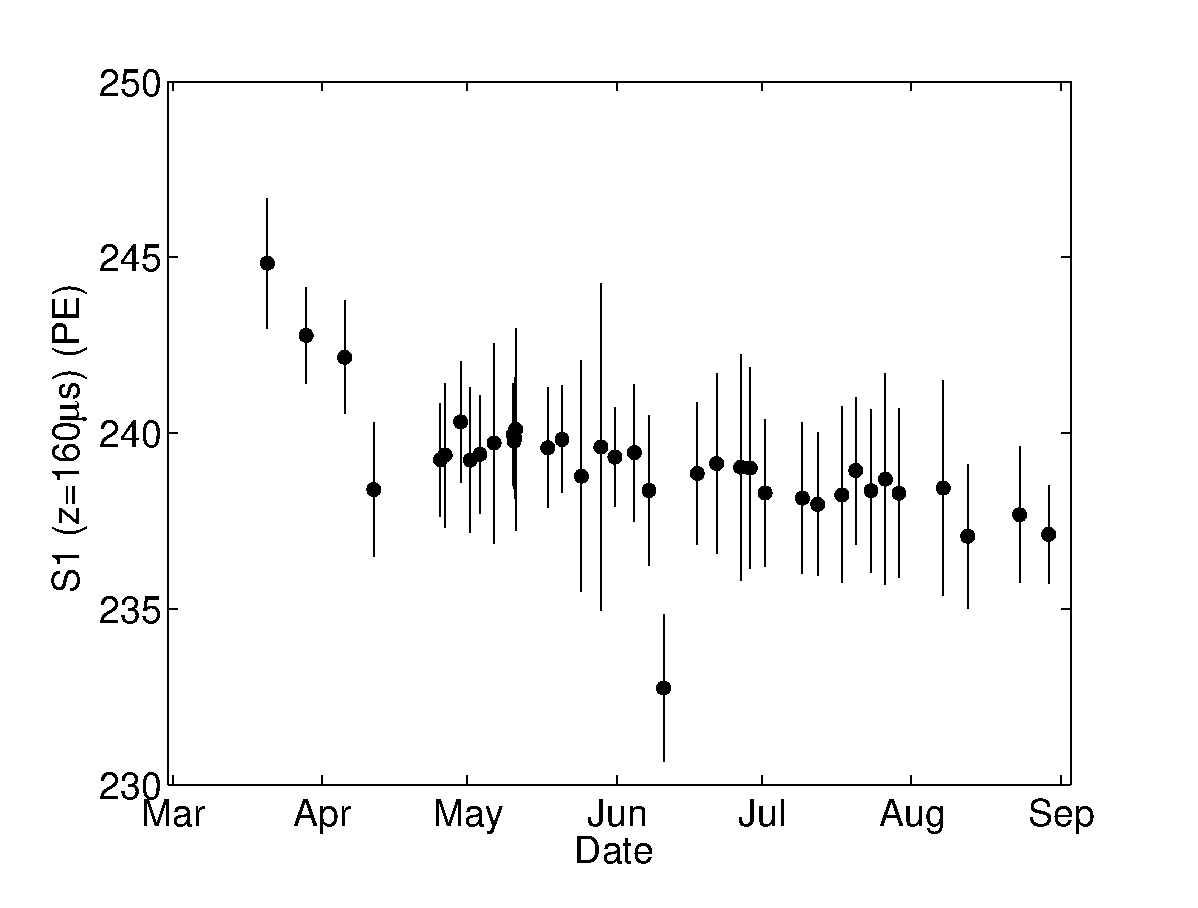
\includegraphics[width=80mm]{Chapter_XYZ_Corr/Thesis_Corr_Plots/s1_center_fig_2.eps}
\caption{Measured response of to light from \KrCal calibrations at the center of the LUX detector over the corse of the LUX science run in 2013.}
\label{fig:S1_center_time}
\end{figure}





